\documentclass[tikz,border=2pt]{standalone}
\usepackage{tikz}
\usepackage{pgfplots}
\usetikzlibrary{intersections}
\usetikzlibrary{positioning}
\usetikzlibrary{graphs}
\usetikzlibrary{backgrounds}
\usetikzlibrary{plotmarks}

\begin{document}

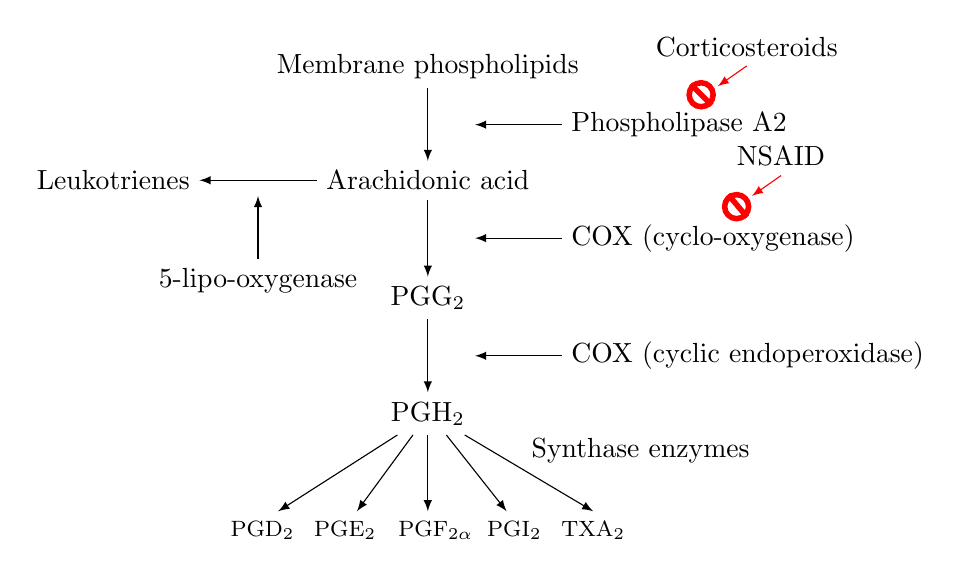
\begin{tikzpicture}
\node[](T1)at(0,0){Membrane phospholipids};
\draw[-latex,black,](T1)--coordinate(V1)(0,-1.2)node[black,below](T2){Arachidonic acid};
\draw[-latex,black,](T2)--coordinate(V2)(0,-2.67)node[black,below](T3){PGG$_2$};
\draw[-latex,black,](T3)--coordinate(V3)(0,-4.14)node[black,below](T4){PGH$_2$};

\draw[-latex,black](T2)--coordinate(ST3a)++(-2.9,0)node[left,black](T3a){Leukotrienes};
\draw[shorten <=2mm,latex-,black](ST3a)--++(0,-1)
node[below,black]{5-lipo-oxygenase};
\draw[shorten <=6mm,latex-,black](V1)--++(1.7,0)
node[right,black](PH){Phospholipase A2};
\draw[shorten <=6mm,latex-,black](V2)--++(1.7,0)
node[right,black](COX){COX (cyclo-oxygenase)};
\draw[shorten <=6mm,latex-,black](V3)--++(1.7,0)
node[right,black](COX2){COX (cyclic endoperoxidase)};
%%
\node[draw=red,shape=circle,line width=2pt,
minimum height=3.05mm,inner sep=1pt] (C1)at([yshift=1mm]PH.45){};
\draw[red,line width=2pt](C1.315)--(C1.135);
\draw[shorten <=0.5mm,red,latex-](C1.25)--++(35:0.5)node[above,black]{Corticosteroids};
%
\node[draw=red,shape=circle,line width=2pt,
minimum height=3.05mm,inner sep=1pt] (C2)at([yshift=1mm]COX.45){};
\draw[red,line width=2pt](C2.315)--(C2.125);
\draw[shorten <=0.5mm,red,latex-](C2.35)--++(35:0.5)node[above,black]{NSAID};

\def\x{-5.65}
\path[green](-2,\x)--(2,\x)coordinate(PO);

\draw[black,-latex](T4)--(T4|-PO)
node[black,below,font=\footnotesize,xshift=1mm]{PGF$_{2\alpha}$};
\draw[black,-latex](T4.215)--(-1.9,\x)
node[black,below,font=\footnotesize,xshift=-2mm]{PGD$_2$};
\draw[black,-latex](T4.235)--(-0.9,\x)
node[black,below,font=\footnotesize,xshift=-1.5mm]{PGE$_2$};
\draw[black,-latex](T4.311)--(1,\x)
node[black,below,font=\footnotesize,xshift=1mm]{PGI$_2$};
\draw[black,-latex](T4.330)--node[right=4mm,black,pos=0.2]{Synthase enzymes}(2.1,\x)
node[black,below,font=\footnotesize,xshift=0mm]{TXA$_2$};
\end{tikzpicture}
\end{document}